% !TeX root = SketchFace.tex

\section{Deep Network for Sketch-Photo Translation}
\label{sec:network}

\begin{figure*}
	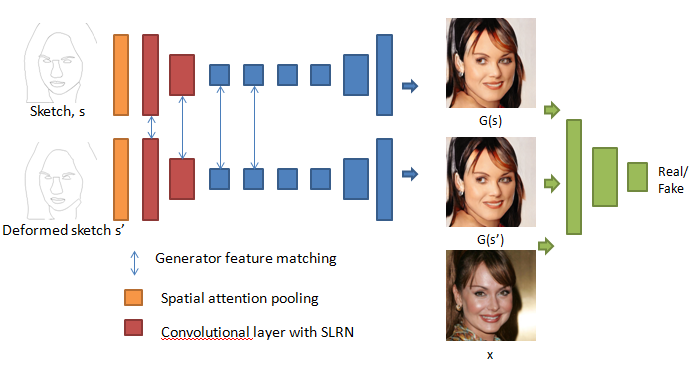
\includegraphics[width=0.9\textwidth]{figs/architecture}
	\caption{The architecture of our model.}
	\label{fig:architecture}
\end{figure*}
%
%%%%%%%%%%%%%%% Section Openning %%%%%%%%%%%%%%%%%%%%%%%%%%%%%%%%
In this paper, we propose a sketch-to-photo translation model that is robust to hand-drawn sketches. In order to handle hand-drawn sketches, we design a novel spatial attention pooling (SAP) module to adaptively adjust the spatial-variant balance between \textit{the realism} of the synthesized face image and \textit{the correspondence} between input sketch and the edges in synthesized image. 
We arrange this section as follow. We first introduce the dataset we construct for our model in Subsection~\ref{subsec:algorithm_data}.
Then we describe the architecture of our model in Subsection~\ref{subsec:algorithm_overview} and the proposed SAP in Subsection~\ref{subsec:algorithm_sap}.
At last we discuss losses applied in our model in Subsection~\ref{subsec:algorithm_loss} and the multi-stage training schedule in Subsection~\ref{subsec:algorithm_training}.




%%%%%%%%%%%%%% Face Sketches and Stroke Deformation  %%%%%%%%%%%%%%%%%%%%%%%%%%%%%%%%%%%%%%%
\subsection{Face Sketches and Stroke Deformation}
\label{subsec:algorithm_data}
% !TeX root = SketchFace.tex


Paired face sketch-photo dataset is required for supervised sketch-to-face translation methods.
Since there exits no large-scale paired face sketch dataset, the training face sketches used by existing methods are generated from face image dataset, e.g. CelebA-HQ face dataset, using edge detection algorithm such as HED~\cite{HED}.
%
However, the sketches generated by edge detection algorithm are sometimes incomplete or \td{other problems}. 
\td{Discuss the advance of make-edges over edge maps and contours}
\cxj{I would say the edge maps are quite different from handdrawn sketches, not because of the incompleteness.}
\rmv{ Although CSAGAN~\cite{CSAGAM} applied self-attention mechanism to alleviate the incompleteness problem, the others remains. Therefore we use another method to generate clearer and complete sketches from face images.}

~\cite{pix2pixHD} introduce another method to generate sketches from face images. Given a face image, the face landmarks are detected using an off-shelf landmark detection model. A new kind of sketch, denoted as \textit{face contour}, is obtained by connect specific landmarks. Sketch-to-face model trained by face contour fail to generalize to hand-drawn sketches with hair, wrinkles or beard. 

The CelebAMask-HQ dataset~\cite{CelebAMask-HQ} provides a face semantic map for each face image in CelebA-HQ dataset. We basically use the boundary map of the semantic map as the sketch of the corresponding face image. Figure~\ref{fig:sketch_data} shows an example of comparison between a sketch generated by edge detector, a face contour and a sketch generated from semantic boundary.
%


\paragraph{Stroke Deformation}
A shortcut of sketches generated from semantic boundary (and those generated by edge detector) is the lines of sketches are perfectly aligned to edges of the corresponding face images. In order to break the edge-alignment and mimic the hand-drawn sketches, we apply a deformation to the lines, similar to that in FaceShop~\cite{FaceShop}. Specifically, we vectorize lines of each sketches using AutoTrace algorithm~\cite{AutoTrace}, and add an offset randomly selected from $[-d, d]^2$ to the control points and end points of the vectorized lines, where $d$ is the maximum offset and we set $d=11$ in our experiments.
%
Both the initial sketches generated from semantic boundary and deformed sketches are used as the input sketches to our model.


\begin{figure}
	\centering
	\vspace{1.0cm}
	\caption{Comparison between a sketch generated from edge detection and from semantic boundary.}
	\label{fig:sketch_data}
\end{figure}


%%% TODO: add semantic map 
\begin{figure}
	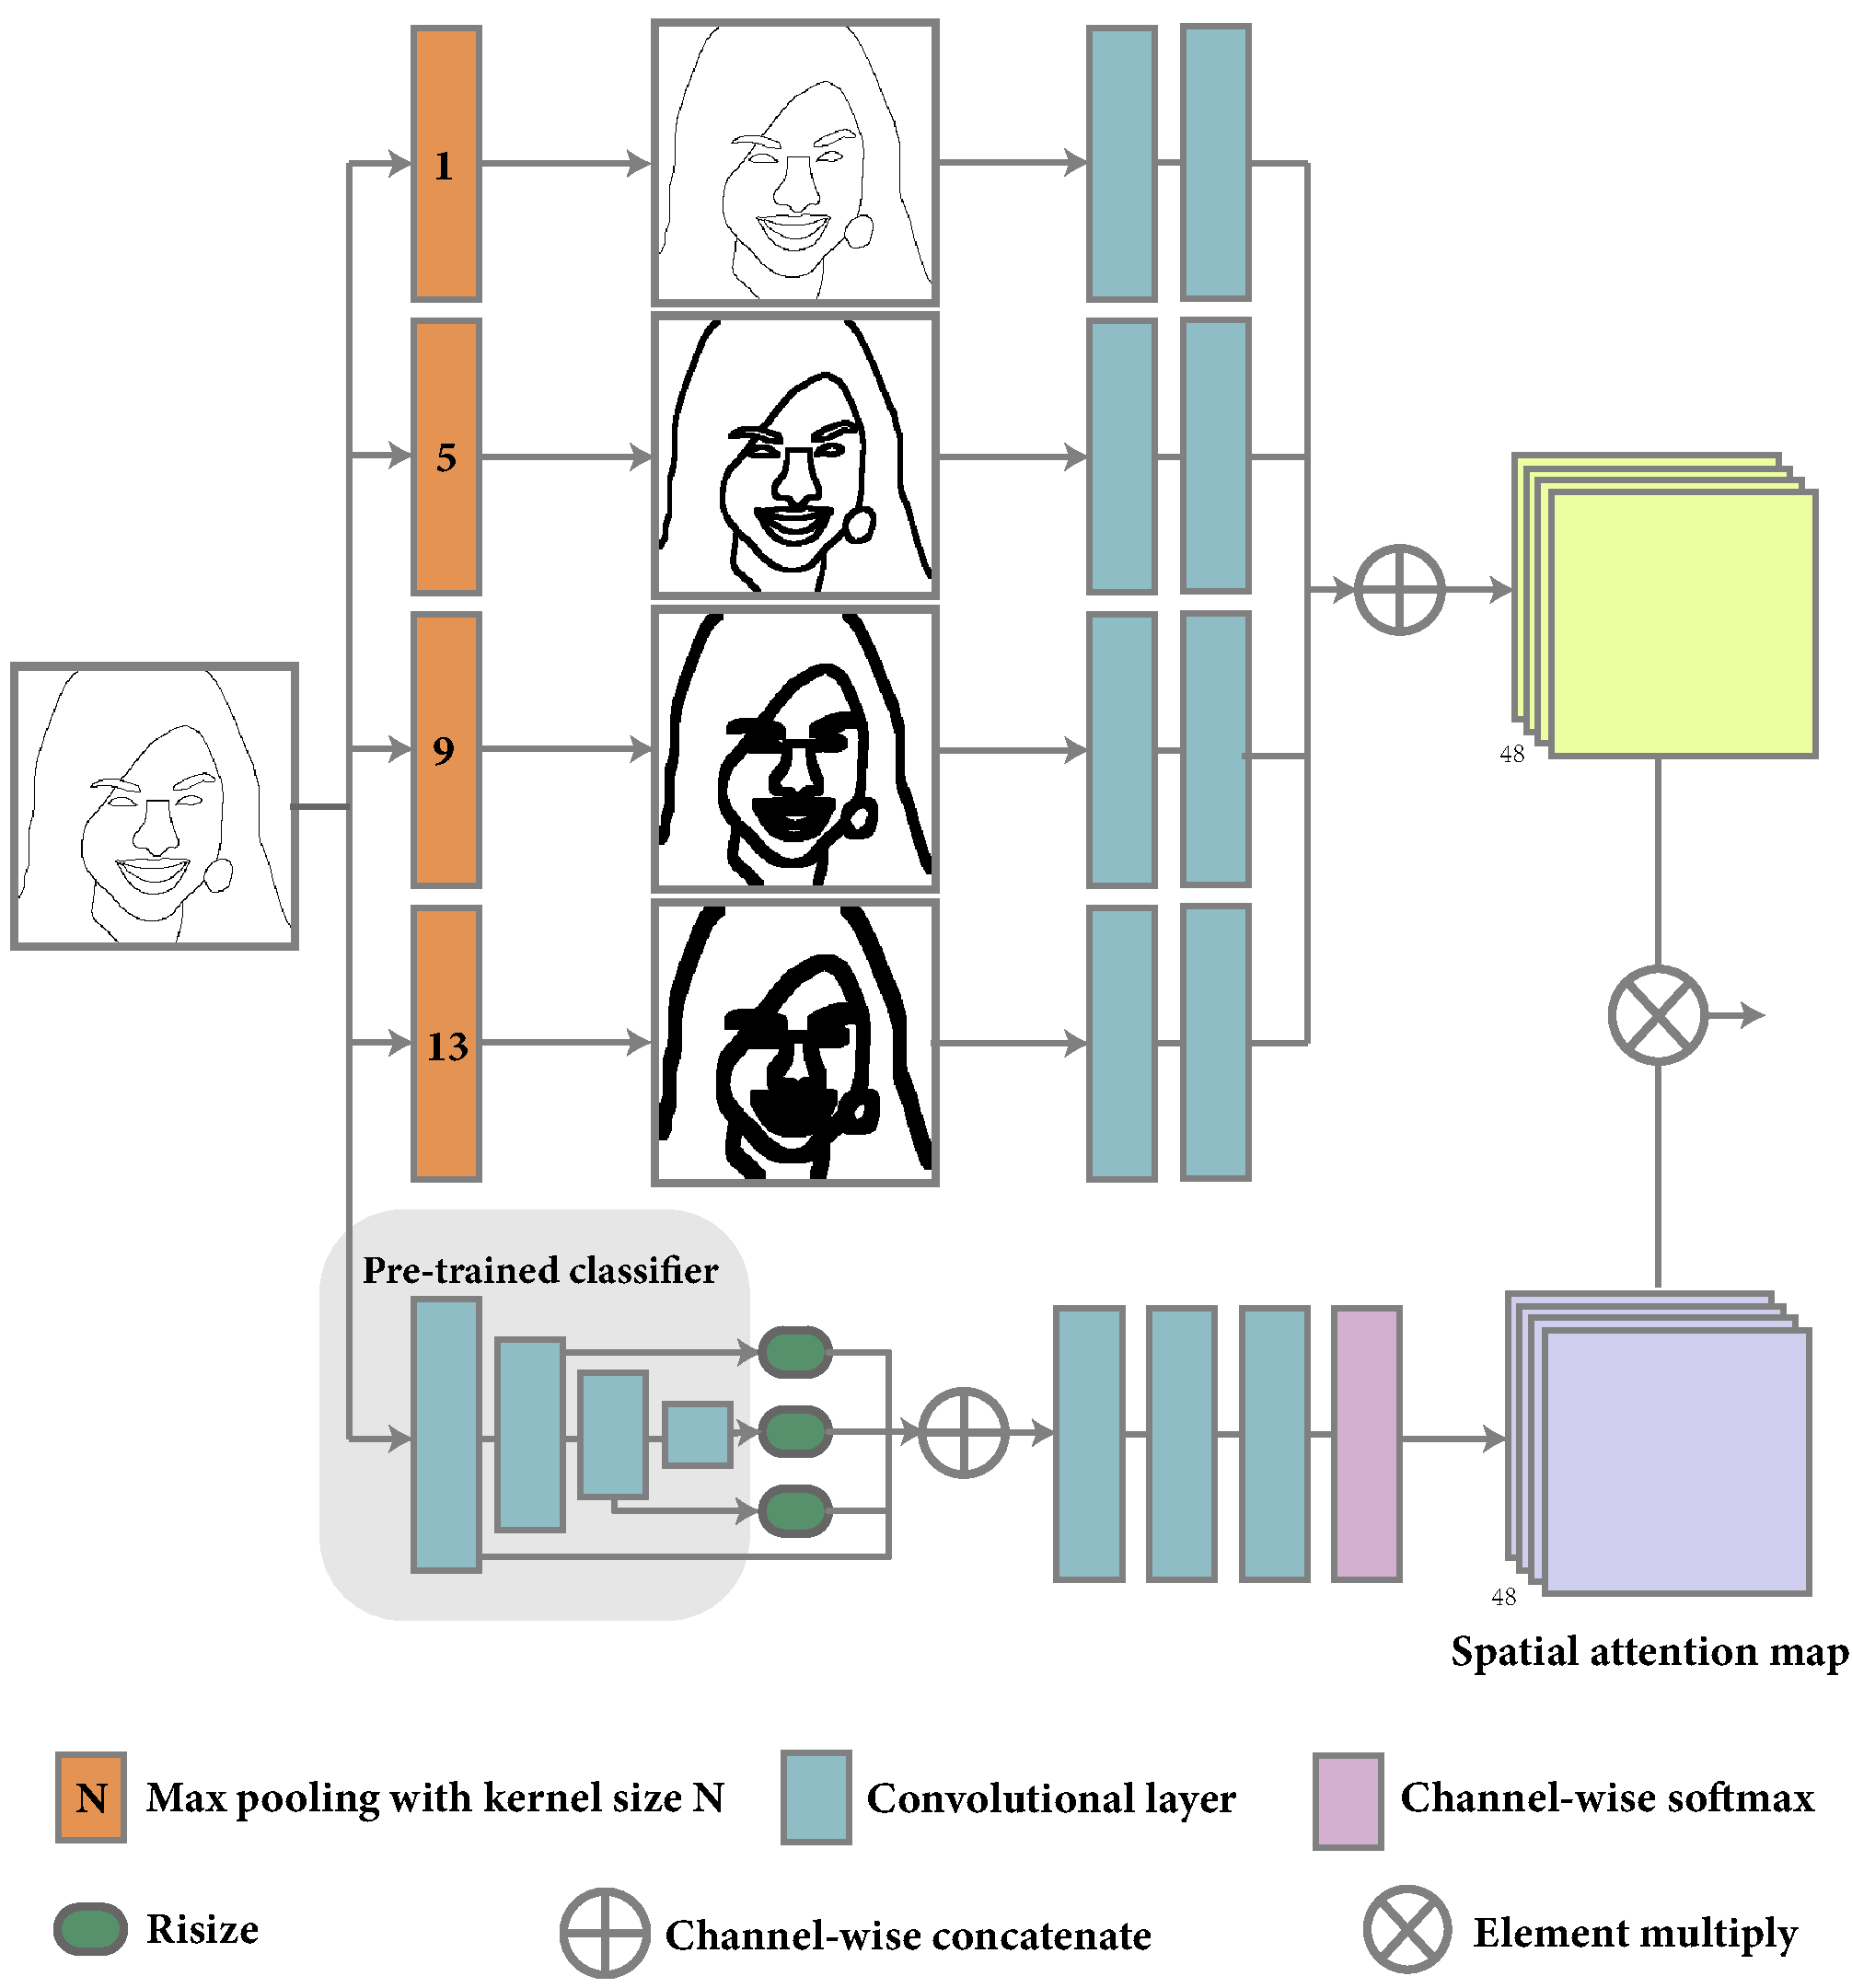
\includegraphics[width=\columnwidth]{figs/sap}
	\caption{Sap}
	\label{fig:sap}
\end{figure}
%
%%%%%%%%%%%%%% Overview  %%%%%%%%%%%%%%%%%%%%%%%%%%%%%%%%%%%%%%%
\subsection{Overview}
% !TeX root = SketchFace.tex
% 

The task of sketch-to-photo translation can be defined as looking for a generator $G(S)$ so that the generated image $I=G(S)$ from a hand-drawn sketch $S$ looks realistic and keeps the shape characteristics for the input sketch.
%
Existing image translation techniques train a neural network as the generator with paired of sketch and photo data $(\mathcal{S}, \mathcal{I})$.
%
Due to the scarcity of real hand-drawn sketches, existing techniques synthesize sketches in a certain style to approximate the sketch set $\mathcal{S}$ from face image set $\mathcal{I}$ to train their generator in an adversarial manner.
The synthesized sketches $\mathcal{S}_{syn}$ are usually well aligned with the face images and present different distributions from hand-drawn sketches $\mathcal{S}$.
These models typically fail to generalize to hand-drawn sketches by common users. 
%


As shown in Figure~\ref{fig:architecture}, $G_m$ is the main generator trained by deformed sketches $S'$, aiming to generate plausible photo-realistic face images from unseen hand-drawn sketches in test stage. 
$G_a$ is an auxiliary generator trained with edge-aligned sketches whose goal is to guide $G_m$ to adaptively sense the line distortion in deformed sketches.


We propose a novel network architecture with a specially designed training strategy to improve the capability of the sketch-based image generator.
%
Figure~\ref{fig:architecture} shows the overview of our method.
%
In order to synthesize a set of sketches $\synS$ that has similar distribution with hand-drawn sketches $\hdS$, we deform the edge-aligned sketches to generate a set of deformed sketches $\dfmS$ to augment the training set.
We propose a novel framework using dual generators from the edge-aligned sketches $\synS$ and the deformed sketches $\dfmS$ respectively.
%
$G_m$ is the main generator trained by deformed sketches $S'$, aiming to generate plausible photo-realistic face images from unseen hand-drawn sketches in test stage. 
$G_a$ is an auxiliary generator trained with edge-aligned sketches whose goal is to guide $G_m$ to adaptively sense the line distortion in deformed sketches.
%
A spatial attention pooling module (SAP) is added before the encoder $E_m$ of $G_m$ to adjust the spatially varying balance between \textit{the realism} of generated images and \textit{the conformance} between the generated image and the input sketch. 
%

The dual generators are trained together under a set of supervision. 
First, for a triplet $(S,S',I)$, both the generators $G_m$ and $G_a$ are trained to produce images $G_m(S')$ and $G_a(S)$ to approximate the real image $I$ under a reconstruction loss $L_{rec}$. 
Second, a multi-scale discriminators $D$ is employed for three combinations of sketch-image pairs to distinguish real face images from generated fake images in both global and local scales. 
By training the dual generators simultaneously with the discriminator adversarially, our main generator $G_m$ effectively captures the spatially-varying stroke distortions and maps it to the manifold of well-drawn sketches to produce realistic face images.


\dlt{

%Both generators are encoder-residual-decoder architectures, including an encoder, several residual blocks and a decoder, which is proven to be effective for generate high-quality images. 
%The generators share weights of the residual blocks and decoders since the high-level features of both generators are supposed to share with each other.



The discriminator is a multi-scale discriminator~\cite{pix2pixHD} which distinguishes real face images from generated fake images in both global and local scales.
For the discriminator, the generated image $G_m(S')$ and $G_A(S)$ concatenated with their input sketch $S$ and $S'$ respectively are treated as fake samples while a real face image sampled from real face distribution concatenated with its corresponding sketch is regarded as a real sample. 
%
%In the adversarial training stage, the generator and the discriminator are updated alternately.

In order to guide the model with SAP to be tolerant with line distortion of deformed sketches, we design a novel generator feature matching loss for our task, besides the adversarial loss, the reconstruction loss and the discriminator feature matching loss. The model is trained in a multi-stage training schedule to ensure the convergence of the training.
%



We arrange this section as follow. We first introduce the dataset we construct for our model in Subsection~\ref{subsec:algorithm_data}.
Then we describe the architecture of our model in Subsection~\ref{subsec:algorithm_overview} and the proposed SAP in Subsection~\ref{subsec:algorithm_sap}.
At last we discuss losses applied in our model in Subsection~\ref{subsec:algorithm_loss} and the multi-stage training schedule in Subsection~\ref{subsec:algorithm_training}.
}


%%%%%%%%%%%%%% Spatial Attention Pooling  %%%%%%%%%%%%%%%%%%%%%%%%%%%%%%%%%%%%%%%
\subsection{Spatial Attention Pooling}
\label{subsec:algorithm_sap}
% !TeX root = SketchFace.tex

 
A sketch-to-image model trained with edge-aligned sketch-image pairs tends to generate images whose edges strictly align with the stokes of the input sketch.
When an input hand-drawn sketch is not well-drawn, line distortions in the input sketch damages the quality of the generated face image. 
It is a trade-off between the realism of the generated face image and the correspondence between the input sketch and the output face image.
%
In order to alleviate the edge alignment between the input sketch and the output face image, we propose to relax thin strokes to a tolerance region with various width.
%
A straightforward way is to smooth the strokes to multi-pixel width by image smoothing or dilation. 
%
However, the capacity of this hand-crafted way is limited, because the uniform smoothness for all positions of the whole sketch violate the unevenness of hand-drawn sketches on depicting different facial parts. 
%
We argue that the balance between the realism and the correspondence differs from one position to another across the face image. Therefore, the relaxation degree should be spatially varying. 


Based on the discussion above, we propose a new module, called spatial attention pooling (SAP), to adaptively relax the strokes in the input sketch to spatially varying tolerance regions. 
%
A stroke with a larger width indicates the less restrict between this stroke and the corresponding edge in the synthesized image. The widths are controlled by the kernel sizes of pooling operators. However, the kernel size of pooling operator is not trainable using back propagation algorithm. SAP applies multiple branches of pooling operators with different kernel sizes to get multiple relaxed sketches with different widths. The relaxed sketches are then fused by a spatial attention layer which spatially adjusts the balance of \textit{realism} and \textit{correspondence}. The module is formulated as follow.

%Let $\mathbf{r}=\{r_i | i=1,2,...,N_r\}$ be a set of relax radius. 
The architecture of SAP is shown in Figure~\ref{fig:sap}.
Given an input deformed sketch $S'\in \real^{H\times W}$, we first pass it through $N_r$ pooling branches with different kernel sizes of $\{r_i, i=1,\ldots, N_r\}$ to get $\P_{i}=Pooling_{r_i}(S') (i=1,\ldots,N_r)$. 
Then we utilize convolutional layers to extract feature maps of $P_i$ separately. These feature maps are concatenated to get a relaxed representation of $S'$, denoted as $R$:
%
\begin{equation}
R=Cat(Conv_1(P_1), Conv_2(P_2),..., Conv(P_{N_r})),
\end{equation}
where $Conv_i() (i=1,\ldots,N_r)$ indicates convolutional layers, $Cat$ is a channel-wise concatenate operator.

On the other hand, we compute a spatial attention map $A$ which controls the relax degrees of all positions by assigning different attention weights to $R$.
A stoke with a large distortion is supposed to be assigned with a large relax degree. Hence, $A$ is supposed to adaptively pay more attention (a large weight) to a $Conv_i(P_i)$ with a large kernel size in the areas with large line distortions.
%
A straightforward way to get $A$ is passing the input sketch through a few convolutional layers and these convolutional layers are trained to detect the areas with line distortions. However, we found the a few convolutional layers are insufficient to learn to detect line distortions directly. Therefore, we introduce a two-class classifier to ease the detection. Specifically, we pre-train a fully-convolutional two-class classifier $C$ with three convolutional layers to distinguish sketches from deformed sketches. Then we utilize this pre-trained classifier to extract features of the input sketch $S$ to get ${C_i(S), i=1,2,3}$, where $C_i(·)$ denotes the $ith$ feature maps extracted by $C$. These feature maps from classifier emphasize the differences between sketches and deform sketches. We resize and concatenate these feature maps, and pass them through three convolutional layers to get the spatial attention map:
%	
\begin{equation}
A=Softmax(Conv([C_1, Up_2(C_2), Up_4(C_3)])), 
\end{equation}
%
where $Up_2$ and $Up_4$ indicates $2\times$ and $4\times$ upsampling, Conv(·) indicates three cascaded convoutional layers, and $Softmax(·)$ is a softmax layer computed over channels to ensuring that for each position of $A$, the sum of weights of all channels equals to $1$.

At last, the output SAP is computed as:
%	
\begin{equation}
SAP(S')=A*R,
\end{equation}
%
where $*$ is element-wise multiplication.

%










%%%%%%%%%%%%%% Losses  %%%%%%%%%%%%%%%%%%%%%%%%%%%%%%%%%%%%%%%
\subsection{Losses}
\label{subsec:algorithm_loss}
% !TeX root = SketchFace.tex

Our model consists of two generators, $G()$ for edge-aligned sketch $S$ and $G'()$ deform sketch $S'$, and one discriminator $D()$. Loss functions and objective of our model are discussed as follow.

\paragraph{Reconstruction Loss}
For either generator, a reconstruction loss is applied to guide the generated image to get close to its corresponding real image $x$.

\begin{equation}
\label{eqn:loss_rec}
\begin{aligned}
\mathcal{L}_{Rec}(G, G') &=\mathbb{E}_{(S, x)\sim p_{data}(S,x)\|G(S) - x\|_1} \\
&+ \mathbb{E}_{(S', x)\sim p_{data}(S',x)\|G'(S') - x\|_1},
\end{aligned}
\end{equation}

\paragraph{Adversarial Loss}
The multi-scale discriminator~\cite{pix2pixHD} $D$ consists of three sub-discriminators $D_i, i=1,2,3$.  The adversarial loss for $G$ and $D$ is defined as:
\begin{equation}
\label{eqn:new_loss_adv}
\begin{aligned}
\mathcal{L}_{adv}(G;D)&=\frac{1}{3}\sum_{i=1}^{3}E_{(\bm{S},\bm{x})\sim p_{data}(\bm{S},\bm{x})}\big[\log D_i(\bm{S},\bm{x})\big] \\
& + E_{\bm{x}\sim p_{data}(\bm{S})}\Big[\log \Big(1-D_i \big(\bm{S},G(\bm{S})\big)\Big)\Big].
\end{aligned}
\end{equation}
The adversarial loss for $G'$ and $D$ is defined similarly.

\paragraph{Discriminator Feature Matching Loss} Similar to pix2pixHD\cite{pix2pixHD} and lines2face~\cite{Lines2Face}, we use a discriminator feature matching loss as the perceptual loss, which is designed to minimize the error between generated image and real image in feature space. Here discriminator feature matching loss use the discriminator as the feature extractor. Let $D^q_i()$ be the output of $q$th layer in $D_i$. This loss for $G$ and $D$ is defined as:
\begin{equation}
\label{eqn:feature_matching_loss}
\mathcal{L}_{fm}(G)=\frac{1}{3N_Q}\mathbb{E}_{(\bm{S},\bm{x})\sim p_{data}(\bm{S},\bm{x})}\sum_{i=1}^{3}\sum_{q\in Q} \frac{1}{n_i^q} \|D^q_i(G(\bm{S}))-D^q_i(\bm{x})\|_1 ,
\end{equation}
where $Q$ is the selected layers of discriminator for computing this loss, $NQ$ is the number of elements in $Q$, $n^q_i$ is the number of elements in $D^q_i$.
Also, the discriminator feature matching loss for $G'$ and $D$ is defined similarly.

\paragraph{Generator Feature Matching Loss}
Similar to discriminator feature matching loss which is designed to minimize the error between generated image and real image in feature space, we propose a novel generator feature matching loss that aims to minimize the error between the presentations of $S$ and $S'$ in generator feature space. Let $G^t()$ and This loss is calculated as:

\begin{equation}
\label{eqn:loss_GFM}
\mathcal{L}_{GFM}(G, G')=\mathbb{E}_{(S, S')\sim p_{data}(S, S')} \frac{1}{N_T} \sum_{q\in Q}  \frac{1}{|G_q|} \|G_q(S)-G_q(\tilde{S}) \|_1,
\end{equation}


Let $G_q(\cdot)$ produces the feature maps of the $q$-th layer in the generator $G$.
%
Given an input sketch $S$ and the corresponding deformed sketch $\tilde{S}$, we compute the generator feature matching loss as:


%
where $|G_q|$ denotes the number of elements in $G_q(\cdot)$, $Q$ indicates a set of the selected generator layers for computing this loss and the size of $Q$ is $N_Q$. 
We select \td{the xxx layers} of the generator in our experiments.

Besides the generator feature matching loss $\mathcal{L}_{GFM}(G)$, for generator $G$ and multi-scale discriminator $D={D_k | k=1,2,...,N_D}$, the adversarial loss $\mathcal{L}_{GAN}(G, D)$ and the discriminator feature matching loss $\mathcal{L}_{DFM}(G, D)$ are computed as the same form as those in pix2pixHD~\cite{pix2pixHD}. \td{Discussion: add equations of these two losses or not}
%
The objective of the proposed model is:

\begin{equation}
	\label{eqn:new_minmax_game}
	\min_G \max_{D} \mathcal{L}_{GAN}(G, D)+\lambda \mathcal{L}_{DFM}(G, D) +\mu \mathcal{L}_{GFM}(G).
\end{equation}

where $\lambda$ and $\mu$ are the weights for balancing different losses. We set $\lambda=\td{xxx}$ and $\mu=\td{xxx}$ in our experiments.

%%%%%%%%%%%%%% Traning Schedule %%%%%%%%%%%%%%%%%%%%%%%%%%%%%%
\subsection{Training Schedule}
\label{subsec:algorithm_training}
% !TeX root = SketchFace.tex

In order to train our model more stably, we introduce a multi-stage training schedule. At the first stage, we use edge-aligned sketches and real images to train $G_a$ and $D$ without loss function related to $G_m$. At the second stage, we train SAP and the encoder of $G_m$ and $D$ from scratch while fixing weights of other parts. Note that the residual blocks and the decoder of $G_m$ share weights with those of $G_a$ and are kept unchanged in this stage. At the last stage, we finetune the whole model. 
